\setcounter{chapter}{ 6 }
\chapter{\textbf{GC Station, Part 2} }

\subChapterTitle{``Caduceus''} 

\deets{Suko}{Sept 4th, 2012}



Finally Jaya got to punch and shoot things!   \hl{:)}\footnote{\textbf{Rebecca S. }:D  and also  XD  
Other people got to shoot things as well! \textsubscript{09/12/12 10:44pm}}



Also, if you want to see what people have added/changed, go to File → See Revision History.  It's pretty handy to quickly spot where the changes have been made.



\noindent\hrulefill





\jumpHeadline{GC Station} 


\sceneHeadline{The Shaft }

We pick up right after the end of last session.  Jayce tells us that we want to head down the middle tunnel, and it will lead us to The Shaft \textit{{[}The Shaft: 9 Tokens enter the threat pool{]}}.



Jaya heads straight for the tunnel, with Hayley and Oliver following.  \hl{Jonah lingers to talk with Jayce, thanking him for his help, and trying to make their parting less tense than it was after the fight.}\footnote{\textbf{Nathaniel Ford }More important than realized at the time... \textsubscript{11/07/14 7:49pm}}



At the end of the tunnel is a fairly large open area with several stone piers with gravel below.  There are four smaller holes/tunnels at the end of the piers.  There is a great deal of rubble and the ceiling has at least partially collapsed.  There is a rupture in the ground that cuts across the piers and leads toward a large hole/break in the wall on the left side.  



Jonah investigates to the left, while Jaya and Hayley investigate the smaller tunnels. There are tracks that lead into the tunnels and they seem to terminate not far from the opening.  Jonah sees that the collapsed area leads into a slope that goes downward.  At the end he can faintly see the glitter of what seems like glass (though slightly strange and likely a material he doesn't recognize) and the faint grey sheen of concrete.



The squad regroups and heads down the slope that Jonah found.  It is not easy going, as it is a steady incline and slicked with the pervasive dampness, and Oliver lags behind.



About 100 meters down the incline there is another tunnel that intersects this one, but this one heads straight down.  The incline continues on the other side of the intersection.  There are no walls or fences to keep someone from tumbling straight into The Shaft if they are not careful.  



Jaya leans over the edge and spits into darkness to see if she can tell how deep it is \textit{{[}}\textit{\textbf{???}}\textit{: }\textit{\hl{12 Tokens enter the threat pool}}\footnote{\textbf{q.google }What was the name of the Threat? \textsubscript{09/06/12 3:49pm}}\textit{{]}.}   A colony of bats swarms out of the darkness \textit{{[}Challenge: Argh!  Bats!{]}}.  Jaya flips out, grabbing bats out of the air and stomping on them and flailing around with her truncheon, nearly smashing Hayley in the face, but we manage to survive the bats.  



Once the bats are gone, we lower a flashlight on a rope and see that The Shaft is over 100 feet deep and we can't see the bottom of it.  It is peppered with twisted bits of metal and rebar embedded in the sides, as if something used to be attached but was removed/torn off.  About 75 feet down, there looks like a tunnel or opening in the side.



Hayley climbs down but misses a handhold \textit{{[}Refresh: Athletics{]}} and falls \textit{{[}Challenge: Stop Hayley from falling{]},} and the rope that she tied off at the top gets untied and starts slithering down after her.  Luckily Oliver is able to hang onto the rope long enough for her to maneuver to the opening in the side and climb in.  The rope falls into The Shaft, although the other end is still tied to Hayley so we don't lose it entirely.  Jaya scolds everyone loudly about their near miss, and as Jonah tries to quiet her down, some nearby masonry crumbles from all the noise.



Hayley reports that in the opening is a door, a large metal one, with SAC-01 on it.  There's a small terminal next to the door that looks like it needs an access card of some kind.  The terminal seems to be without power.  Two Notice challenges go back to the pool.  Oliver calls T\hl{renton, who tells Oliver retrieve the card that is in Hayley's uniform's front breast pocket.}\footnote{\textbf{Nathaniel Ford }Trenton, fondling remotely \textsubscript{11/07/14 7:52pm}}Alas, such suave moves are impossible given the current circumstances, so Hayley retrieves the card herself and inserts it into the terminal.  Nothing happens.



Hayley is attacked by a small vicious creature, like a \hl{spider monkey}\footnote{\textbf{Rebecca S. }I \textless 3 monsters!  I think towards the end of the whole scene, their descriptions were revised to be more like ``spider rats''?  Or am I making that up...? \textsubscript{09/12/12 10:37pm}}\footnote{$\rightarrow$\textbf{Suko T }When Hayley freaked out, Nate said that in Hayley's eyes, the monkeys looked like a horrible cross between humans and rats.  Does that sound familiar? \textsubscript{09/13/12 5:07pm}}\footnote{$\rightarrow$\textbf{Nathaniel Ford }Well, they had tails and the size of rhesus macaques, but faces and hair more akin to sewer rats. \textsubscript{09/13/12 5:08pm}}\textit{{[}Challenge: Dodge Killer Monkey{]}}.  She dodges and manages to shove it over the side of the ledge, but it grabs onto the rope that is still tied around her waist, and several more creatures come up over the edge and attack.



At this point Trenton helpfully adds that the card will take about 3-4 minutes to work.  When the light on the dongle turns green, it will work.



But we are all a bit distracted by the \textit{{[}Challenge: Swarm of Killer Monkeys{]}}.  Jaya and Oliver successfully chase them off, while Hayley screams in terror and curls up in a sobbing ball \textit{{[}Refresh: Conditioned{]}}.  Oliver is likewise disturbed by the creatures and keeps firing even long after the creatures are gone \textit{{[}Refresh: Hardened{]}.}  Jonah is distracted by the frenzy and fails to notice the falling debris, now a significant stream of dust, dislodged by the loud noise of gunfire \textit{{[}Refresh: Vigilant{]}}.



The light on the dongle turns green and door by Hayley slides open.  Behind the door is a corridor lit with blue light.  Jaya orders Hayley to find something to block the door open.  All Hayley can think of is her Uniform backpack so she removes it \textit{{[}Refresh: Uniform{]}} and places it in the doorway (she removed the rifle and clipped the flashlight and radio to her uniform, but left everything else).  Jaya then orders Hayley to climb back up to where they are and carry the rope so they can get down.  Hayley ties off one end of the rope to some metal bit near the door and ties the other around her waist. She forgets to grab the card key \textit{{[}Refresh: Ladies' Maid{]} }and starts climbing up.



When she reaches the top, they untie the rope from her and Jonah fastens it to some metal bit stuck in the wall.  Jaya climbs down first.  She almost makes it but then makes the mistake of looking down \textit{{[}Challenge: Mental Anguish{]}}.  The darkness yawning below her is terrifying but she gives herself a pep talk and manages to get the rest of the way to the door without falling.  Oliver goes next and makes it halfway before the pain in his rope-burn damaged hands starts getting so intense it's hard to grip the rope \textit{{[}Refresh: Arm Strength{]}}.  At the same time the rope starts shaking a bit, making it even harder to hang on {[}\textit{Challenge: Hang on!{]}}.  The precarious situation actually helps him focus and he grits through the pain to climb the rest of the way to the door.   With an ease that speaks of long practice at this obscure skill, Hayley scampers quickly down the rope.  Jonah follows quickly, not wanting to stress the rope and anchor any more than necessary.  He almost reaches the door just as the rope goes slack briefly and a large chunk of rock plummets past him, just barely missing his head \textit{{[}Challenge: Vertigo{]}}.  He also manages to hang on and make it to the door safely but with an injured wrist \textit{{[}Flaw 1: Sprained Wrist{]}}.



\jumpHeadline{SAC-01 } 


\sceneHeadline{Hallways }

With the squad reassembled, we head into the corridor.  As soon as we set foot inside, the blue light changes to red and the door begins to close.  Hayley grabs the key card and Jaya grabs Hayley's backpack and hustles everyone inside.  The rope is abandoned outside.



Hayley helps bandage Jonah's injured wrist \textit{{[}Medkit 1 to reduce Sprained Wrist Flaw to 0{]}.}  She shows him a good way to wrap the bandages to allow for at least some limited movement, explaining that she learned to do that because sometime she had to do tests while still recovering from... something.  She doesn't specify what but gestures vaguely at Jonah's bandaged wrist.  When \hl{Jonah asks what she means by ``tests}\footnote{\textbf{q.google }It's more like ``Wait, what, \_tests\_, they made you take \_tests\_?'' but not coherently enough due to be clear due to the pain and time pressure. \textsubscript{09/06/12 3:55pm}}'', she just shakes her head. \textit{{[}Challenge: Notice something during bandaging{]}}.  \textit{{[}OOG: Ion gets pulled into hallway to be told something super sekrit{]}}.



Jaya gets everyone moving again down the corridor, which opens up into a small room with a desk, a chair and two doors.  One door has a funny symbol of a pole with a weird twisty thing around it and wings coming off of the top {[}OOG: It's a caduceus{]}.  The other door has a circle with a grid through it and surrounded by leaves.



Jonah and Oliver argue over what the symbol means \textit{{[}Challenge: What is a caduceus?{]}.}  Jonah recognizes it from the book that Dr. Gerhauser loaned him and believes it has to do with guts around a spine.  \hl{Oliver insists that it has to do with replacing body parts.}\footnote{\textbf{Adam Kenney }Due to a Flaw he picked up from the ``What is a caduceus?'' challenge. \textsubscript{09/06/12 8:16pm}}\footnote{$\rightarrow$\textbf{Suko T }I definitely saw that change, it was funny to see Oliver get all excited about something, especially something like this. \textsubscript{09/07/12 12:26am}}  \hl{Jaya scoffs at such technologies, saying they don't exist}\footnote{\textbf{Rebecca S. }thank goodness she was wrong... \textsubscript{11/10/14 6:19am}}\footnote{$\rightarrow$\textbf{Nathaniel Ford }You don't have to thank an abstract concept. Rook would be happy to accept your gratitude... \textsubscript{11/10/14 4:44pm}}.  Oliver says that they were done in the past, there are records in history.  Hayley had started to nod at Oliver's first statement but then looks surprised at Jaya and Oliver's subsequent statements.  Her hesitant attempts to correct them go unnoticed \textit{{[}OOC: Unless someone thinks their character would notice even if they didn't as a player{]}}.



Oliver adds that it may have to do with ``genetics'' too, which he offhandedly mentions came up in a discussion he had with Dr. Gerhauser.  When Jonah presses him for more info, Oliver waves him off and says it's not important.



Hayley places the card in the terminal by the caduceus door and we wait.  The faint sounds of a voice can be heard through the door.  We can't understand it so Oliver radios Trenton and sees if he can make it out.  After teaching us to make a primitive amplifier (a cup on the door!) Trenton says that the voice is speaking a language he doesn't know, and then deliberately provokes Jaya.



Jaya kicks the door in frustration, just as the light on the card turns green and the door opens.  Hayley grabs the card again and the squad heads down the corridor.



The corridor opens out into a round open area with a ring of nicely appointed rooms with glass walls and doors facing inward.  In the center is a nice spiral staircase going down and we can see other floors below. 



\textit{{[}Challenge: Figure out which rooms to search{]} } Hayley draws on her experience with Citizen's households and offices and realizes that these rooms on this floor are just secretarial or for show.  What we want is probably on a lower floor.  Oliver does not hear her and starts immediately searching the desks on this floor \textit{{[}Refresh: Focused{]}.}  Jaya also starts searching but gets frustrated and starts using her gun to blast open the locks on some of the desk drawers \textit{{[}Refresh: Small Arms{]}.} 


\sceneHeadline{Lower Floor }

Hayley and Jonah head down the stairs \textit{{[}Challenge: Notice the person below{]}}. Hayley notices some movement below: a person-sized figure moving in an odd manner.  She calls Jonah and Jaya's attention to it and they start heading down the stairs (Oliver is still searching the desks and has found several mysterious objects like staplers and ladies' powder compacts).  The second level has rooms with sequential numbers on them.  The third floor is a cafeteria/break area.  The fourth floor has corridors branching off.  The fifth floor has two large doors (like the ones at the front of SAC-09 and SAC-01) facing each other, and four smaller doors placed evenly on the walls between them.  



The voice we'd been hearing is louder in this area and one of the large doors is open.  Jaya yells down the hallway before Jonah can stop her, destroying his opportunity to try to listen for other people in the area \textit{{[}Refresh: Vigilant{]}}.  



The voice changes and begins saying something else in that language that none of us know.  The lights start going out with an ominous thunk, floor by floor, plunging us in relative darkness.  There are some flashing lights in the corridor behind the large open door.



There's a brief argument about which door to go through, which is solved by Oliver insisting on scoping out the open door and Jaya taking the access card and putting it in the terminal next to the closed door.  She sends Hayley to follow Oliver, while she and Jonah watch the other doors.  Jonah peers after them warily, trying to provide cover.



Oliver and Hayley start scouting out the corridor \textit{{[}Challenge: Notice the ``gun''{]}}.  As we approach the first intersection, we can hear the sounds of something wet moving, and the shifting sound of heavy objects.  There is a gooey substance on the floor.  Oliver notices what looks to him like a gun mounted on the ceiling.  He immediately drops to the ground and yanks Hayley down with him, motioning for the others to take cover as well.  Oliver realizes that \hl{his gun is jammed}\footnote{\textbf{q.google }Man, guns jam a lot In The Future.  And this a quality one too. \textsubscript{09/06/12 4:01pm}}\footnote{$\rightarrow$\textbf{Adam Kenney }Bad bullets. \textsubscript{11/08/12 12:13pm}} \textit{{[}Refresh: Crack Shot{]}}.



Oliver sees a woman down the left-hand corridor.  She's taller than Morgan and naked.  She stares back at Oliver with wide eyes.  Not wanting to shoot a defenseless woman, Oliver starts lowering his gun \textit{{[}Refresh: Hardened{]}}, only to realize that the woman has a pistol in her hand and she's swinging it around to fire at him\textit{ {[}Challenge: Avoid getting shot by naked chick{]}}.  Oliver throws himself out of the way to avoid getting shot.  Hayley, meanwhile has gotten tangled up in her rifle and backpack and is just standing there uselessly \textit{{[}Refresh: Athletics{]}}.  Oliver pulls her out of the way.



Peering carefully around the corner, Oliver can see that the corridor has semi-circular doors with glass windows in them on one side and two of them are open.  Across from those are some lockers, and one of them is open.  He can see items in there, like clips and a garment of some kind hanging from the locker door.  The corridor ends, so Oliver knows the woman has to have ducked into one of the two cells that are open.



Jaya joins the party and Oliver tells her to lay down some covering fire while he tries to find the woman.  When Jaya starts firing, a hand comes out of one of the doorways and starts shooting blindly in our direction \textit{{[}Challenge: Shoot gun out of her hand{]}.}  Oliver shoots the gun out of her hand and it goes skittering across the floor.



With Jaya still covering him, Oliver cautiously moves forward.  Now that he's in the corridor, he can see into the windows on the doors that aren't open.  Inside is a purple goo and suspended in the goo are bodies.  They are pretty badly desiccated at this point, and the whole scene is horrific \textit{{[}Challenge: Oh the Horror!{]}.}  Luckily the war has inured Oliver to death and decay, so he fights back the nausea and focuses on finding the woman.  Jaya calls for Jonah to join them and sends Hayley out to watch the other large door and cover their backs.



The naked woman steps out of one of the cells and in her hand is what looks like a grenade.  It is a make unfamiliar to Oliver and Jaya so they can't tell if it's been activated or not.  Oliver tries to talk her down using his \hl{Outgoing personality}\footnote{\textbf{q.google }Was there a challenge here? \textsubscript{09/06/12 4:04pm}}\footnote{$\rightarrow$\textbf{Suko T }Not that I noted, but it could be! \textsubscript{09/06/12 4:19pm}}\footnote{$\rightarrow$\textbf{Adam Kenney }I was trying to make it a challenge, but the scene didn't go that way.  Jaya and Oliver were working at cross-purposes. \textsubscript{09/06/12 8:19pm}}\footnote{$\rightarrow$\textbf{Suko T }No kidding!  It was like a watching a see saw.  We should work on our ``good cop/bad cop'' routine.  Right now we seem to only have mastered ``bad cop/bad cop'' :) \textsubscript{09/07/12 12:32am}} and Jaya attempts to browbeat her into putting the grenade down.  The woman continues to talk to them in another language that we don't know and slowly walks toward them.  They can see now that there's something funny about her skin and although she is in a state of perfect fitness, there is something odd about her.  There is mucus dripping from her nose and face.  Oliver and Jaya back up until they realize the woman is getting near her gun.  They stop and increase their attempts to talk the woman down.  



Jonah, who had just arrived behind them, notices that the woman is going to make a quick break for a console near the lockers \textit{{[}Challenge: Stop the naked chick from hitting the button{]}}.  Oliver shoots the woman in the leg and Jaya rushes her and knocks her out of the way with her truncheon, but not before the woman hits the button and yells something.  The voice that we'd been hearing (we think it may be an automated recording like they have in the train stations) changes yet again and the unintelligible words adopt a slightly more urgent pattern.



Jaya starts beating the woman into submission and the grenade goes tumbling out of the woman's hand.  Oliver, in a moment of selfless sacrifice \textit{{[}Refresh: Hardened{]}}, throws himself on the grenade.  It explodes in a flash of blinding light and then the room starts filling with a noxious smoke.



Meanwhile outside, the light on the access card has turned green and the large door starts grinding open.  As it does, one of the smaller doors opens and a man emerges in a skintight outfit and holding a rifle.  Like the woman, there is something odd about his skin.



When the man hesitates, distracted by Hayley's pretty face, she shoots him with her rifle.  She hits him in the shoulder and sends him stumbling back through the door he came out of \textit{{[}Challenge: Shoot guy in leotard{]}}.  Hayley rushes at him but doesn't get there before the door closes.  Jonah runs back out into the atrium area, alarmed by the sound of gunfire and Hayley's surprised yell but misses seeing the guy.



Jaya wrestles with the woman and punches her into unconsciousness {[}Challenge: Subdue naked chick{]}.  She notices that Oliver is Not Dead Yet\texttrademark and he is staggering to his feet woozily.  Jaya moves to help him stand.  She sees the the burn marks on his stomach and realizes what he had done.  They start choking on the smoke that is filling the corridor.  Oliver reaches down and starts hauling the unconscious woman out of the corridor.  Jaya helps carry the woman out into the area where Hayley and Jonah are.  Hayley tells Jaya that she shot a guy but doesn't think she killed him.  Jaya asks her to try harder next time.


\sceneHeadline{The Archive }

Behind the newly opened door there is a room with a glassed off area.  In the glassed off area there are what looks like card catalogs and a cylinder topped with a dome, with short ladders and a wheel-style lock on top.  The sections are separated by an air-lock-like small room.



Jaya sends Hayley and Jonah into the glassed off area while she zipties the arms and legs of the unconscious woman.  When Hayley and Jonah enter the glassed off area, the voice changes yet again and Jaya knows we must hurry, even though we still can't understand what the voice is saying.



The card catalogs are filled with thin slides of glass.  There are hundreds of them.  Oliver calls Trenton who helps guide Jonah to find slides in the corner drawers that have a discoloring or special marking.  Jonah finds several that have gold markings and he takes all of them, grabbing a handful of the slides next to them to use as padding.  He carefully wraps the whole thing in bandages.



Then Jonah and Hayley open the lock on the top of the cylinder in the room.  The dome takes some effort to open, but they manage to break the seal and as the dome lifts up, a cold thick mist starts pouring out of the container and spilling onto the ground...





\jumpHeadline{Challenges \& Refreshes }  

{
\parskip=0pt
\begin{itemize}
\item Challenge: Argh!  Bats! 2 for each of us except Hayley who got hers bumped to a 3 for Jaya's Refresh of \hl{Truncheon}\footnote{\textbf{Suko T }or was it something else?  I don't have it in my notes \textsubscript{09/05/12 1:06am}}\footnote{$\rightarrow$\textbf{Rebecca S. }Maybe Adrenaline Junkie...? \textsubscript{09/12/12 10:35pm}}\footnote{$\rightarrow$\textbf{Suko T }I don't think so because you used it in the challenge.  But there was a gleeful description of snatching bats out of the air and stomping on them and generally frenzy-ing.  Grim Visage maybe? \textsubscript{09/13/12 5:10pm}}
\end{itemize}

\begin{itemize}
\item Adrenaline Junkie 2 (Jaya) $\rightarrow$ Matched
\item Hardened 2 (Oliver) $\rightarrow$ Matched
\item Uniform 1 (Jonah) $\rightarrow$ Sent back to pool
\item Athletics 2 + Uniform 2 (Hayley) $\rightarrow$ Matched
\end{itemize}

\begin{itemize}
\item Refresh: Truncheon 2 (Jaya).  Die bats die!
\item Refresh: Athletics 2 (Hayley).  I want my gymnasium climbing wall back.
\item Challenge: Stop Hayley from falling 3.  Arm Strength 1 (Oliver) + Dancer 1 (Hayley) + Conditioned 2 (Hayley) → Matched
\item Challenge: Notice (Hayley) something about/around SAC-01 door 1→ Sent back to pool
\item Challenge: Notice  (one of the three still up top) something probably related to what happens next 1 → Sent back to pool
\item Challenge: Dodge Killer Monkey 2: Athletics 2 (Hayley) → Matched
\item Challenge: Swarm of Killer Monkeys 4.  Side Arm 3 (Jaya) + Crack Shot 3 (Oliver) → Matched
\item Refresh: Conditioned 2 (Hayley).  Scary killer rat-human abominations trying to eat me!  Wouldn't \textit{you} scream?
\item Refresh: Hardened 2 (Oliver). Nothing in the war prepared him for creatures like this.
\item Refresh: Vigilant 3 (Jonah).  What do you mean the sky is falling?
\item Refresh: Uniform 2 (Hayley).  Absolutely a bit of cloth weighed down with a handful of protein bars can hold open a heavy duty metal door.
\item Refresh: Ladies' Maid (Hayley). Too scared of Killer Monkeys to remember my duties.
\item Challenge: Mental Anguish 2.  Air of Authority 1 (Jaya) → Sent back to pool
\item Refresh: Arm Strength 1 (Oliver).  Note to self: teach Hayley to tie knots that actually hold.
\item Challenge: Hang on! 2. Hardened 2 (Oliver) → Matched
\item Challenge: Vertigo 2. \textbf{ {\color[RGB]{255,0,0}Flaw: Sprained right wrist 1 (Jonah)} } {\color[RGB]{255,0,0} } → Sent back to pool
\item Medkit 1 (Hayley) → \textbf{ {\color[RGB]{255,0,0}Reduce Flaw: Sprained right wrist from 1 to 0 (Jonah)} }
\item Challenge: Notice something during bandaging 2.  Vigilant 3 (Jonah) → Overcome! \textbf{2 VP (Jonah)}
\item Challenge: What is a caduceus? 2.  Street Medic 2 (Jonah) + Citizen 1 (Oliver) + \textbf{ {\color[RGB]{255,0,0}Flaw: Obsessed with lost medical technologies 1 (Oliver)} }\textbf{ }→ Overcome! \textbf{1 VP (Jonah) + 1 VP (Oliver)}
\item  Challenge: figure out which rooms to search 1. Ladies' Maid 2 (Hayley) → Overcome!  \textbf{1 VP (Hayley)}
\item Refresh: Focused 1 (Oliver).  So many drawers to search!
\item Refresh: Small Arms 3 (Jaya).  Way too f-ing many drawers to search!
\item Challenge: Notice the person below 1.  Bodyguard 1 (Hayley) → Matched
\item Refresh: Vigilant 3 (Jonah).  Will you please stop yelling?
\item Challenge: Notice the ``gun'' 1.  Focused 1 (Oliver) → Matched
\item Refresh: Crack Shot 3 (Oliver).  Dammit this always happens.
\item Refresh: Hardened 2 (Oliver).  Can't shoot a defenseless woman!  Oh crap, she's got a gun.
\item Challenge: Avoid getting shot by naked chick 2.  Arm Strength 1 (Oliver) → Sent back to pool
\item Refresh: Athletics 2 (Hayley). I really need more practice with this rifle.
\item Challenge: Shoot gun out of her hand 4.  Side Arm 3 (Jaya) + Crack Shot 3 (Oliver) → Matched
\item Challenge: Oh the Horror! 1.  Hardened 2 (Oliver) → Overcome! \textbf{1 VP (Oliver)}
\item Challenge: Stop the naked chick from hitting the button 3.  Truncheon 2 (Jaya) + Vigilant 3 (Jonah) + Rifle 2 (Oliver) → Overcome! \textbf{1 VP (Jaya) + 1 VP (Jonah) + 1 VP (Oliver)}
\item Refresh: Hardened 2 (Oliver). Taking one for the team.
\item Challenge: Shoot guy in leotard. Uniform 2 (Hayley) + Gorgeous 3 (Hayley) → Overcome! \textbf{2 VP (Hayley)}
\item Challenge: Subdue naked chick 1.  Grim Visage 2 (Jaya) → \hl{Overcome! \textbf{1 VP (Jaya)}}\footnote{\textbf{Suko T }Is this where Jaya's second VP comes from?  Or did I miss one earlier? \textsubscript{09/05/12 3:08am}}\footnote{$\rightarrow$\textbf{Rebecca S. }D:    I know the total is 2 but I have zero memory of where I got either of them... you're notes \& guesses are better then anything my memory would fabricate.... \textsubscript{09/12/12 10:34pm}}
\end{itemize}
}


\jumpHeadline{VP Totals } 
{
\parskip=0pt

Hayley: 3

Jaya: 2

Jonah: 4

Oliver: 3
}


\jumpHeadline{ Quotes } 


\quotedDialog{
``We can use the rope, right?''

``Not if she falls down the pit and dies.''
}
\extraIndent{ - Jonah and Jaya}



``Not everyone can be 100\%, 100\% of the time!''

\extraIndent{- Jaya}


\quotedDialog{
``Is there a Level 1 Flaw that applies to this?''

``Nerd.''
}
\extraIndent{- Adam and Rebecca}



``The hitting is just the vehicle for intimidation.''

\extraIndent{- Rebecca}


\begin{flushright}
~
\vskip 0em
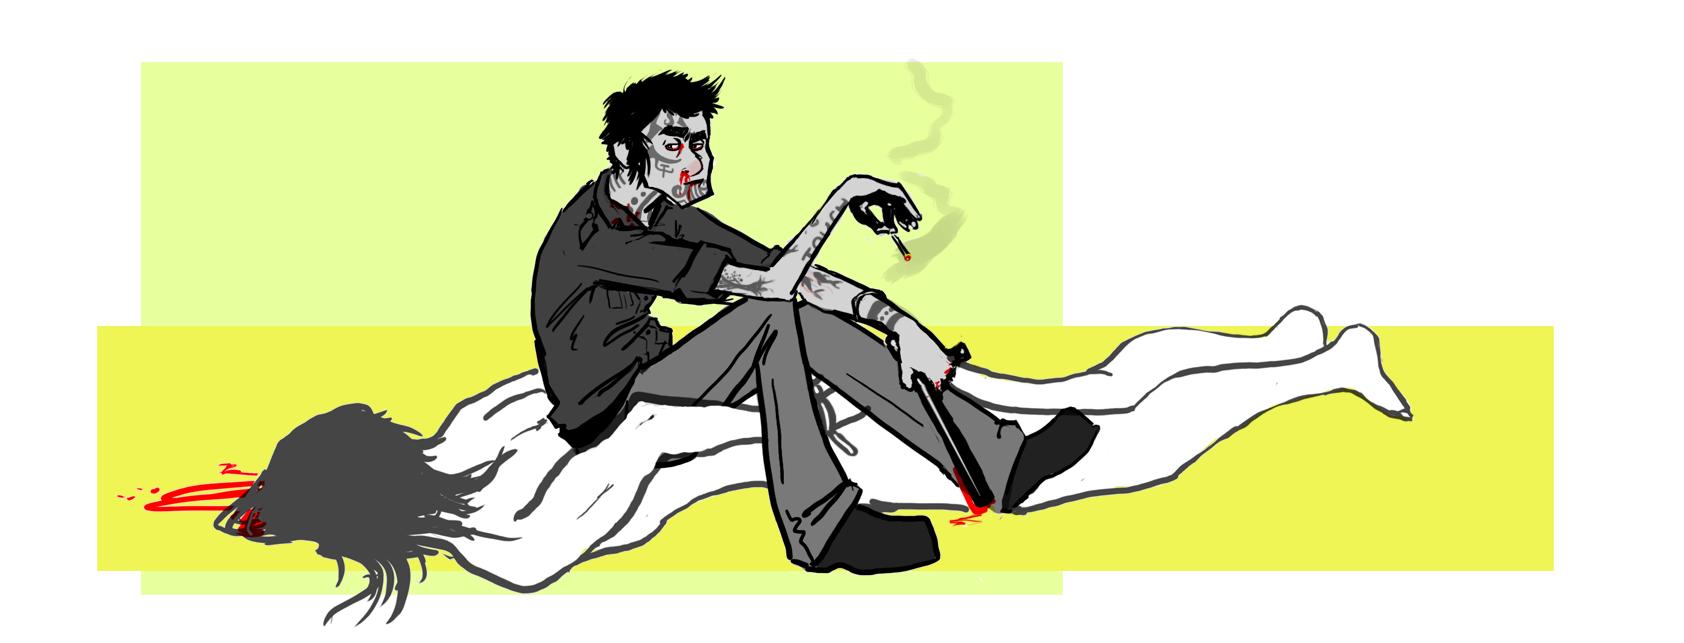
\includegraphics[width=12cm]{img/ch7_jaya_prisoner.png}
\end{flushright}

\vspace{\fill}

\begin{flushright}
\textsubscript{last edited by \textbf{Nathaniel Ford} @ 05/07/15 4:28pm}
% Exported @ 08/22/15 3:51pm
\end{flushright}